\chapter[Proposta]{Proposta}
Este capítulo apresenta detalhes sobre o \textit{framework} proposto neste trabalho de conclusão de curso. O capítulo está organizado em seções. Na seção 4.1, é explanado sobre os requisitos gerais do \textit{framework}. Em seguida, na seção 4.2, é apresentado os objetivos da prova de conceito. Na seção 4.3, é relatado os resultados obtidos até o momento.

\section{Framework para Geração de Teste Unitário}

A proposta deste trabalho é a implementação de um \textit{framework} capaz de dar suporte ao desenvolvedor na tarefa de produzir testes unitários.  Esse suporte deve ser capaz de gerar testes de forma semiautomatizada, visto que o programador deverá incluir no código especificações que guiem o \textit{framework} na criação dos testes unitários. 
\par
\indent A princípio, o \textit{framework} será desenvolvido com o intuito de gerar testes unitários em aplicações escritas em \textit{Grails}, especificamente para as operações básicas conhecidas como CRUD (\textit{create}, \textit{read}, \textit{update} e \textit{detele}). Entretanto, há intenção de evoluir o \textit{framework} para que ele seja compatível com demais métodos, bem como, com outras linguagens de programação. 
\par
\indent Para a implementação do \textit{framework}, será utilizada a linguagem de programação C++, junto com as ferramentas Flexc++ \cite{flexcpp2015} e Bisonc++ \cite{bisoncpp2015}. Essas ferramentas serão responsáveis pela análise léxica do código e \textit{parser} para geração da gramática, respectivamente. A ilustração a seguir fornece uma visão geral da arquitetura do \textit{framework} a  ser construído.
 
 \begin{figure}[h]
    \centering
    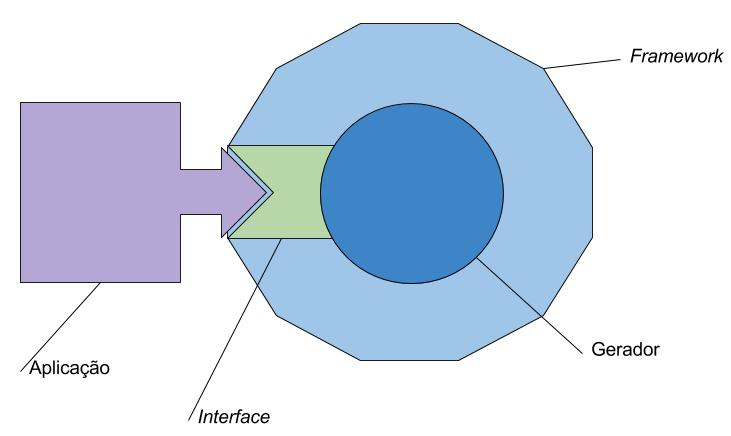
\includegraphics[width=0.7\textwidth]{figuras/estruturaarquitetural.jpg}
    \caption{Visão Geral do \textit{Framework}}
    \label{fig:estruturaarquitetural}
 \end{figure}

 \par
 \indent O \textit{framework} proposto possuirá em seu núcleo um gerador de testes unitários e, em uma camada mais elevada, possuirá uma interface com a função de possibilitar a interação com a aplicação. 
 
   \begin{figure}[h]
    \centering
    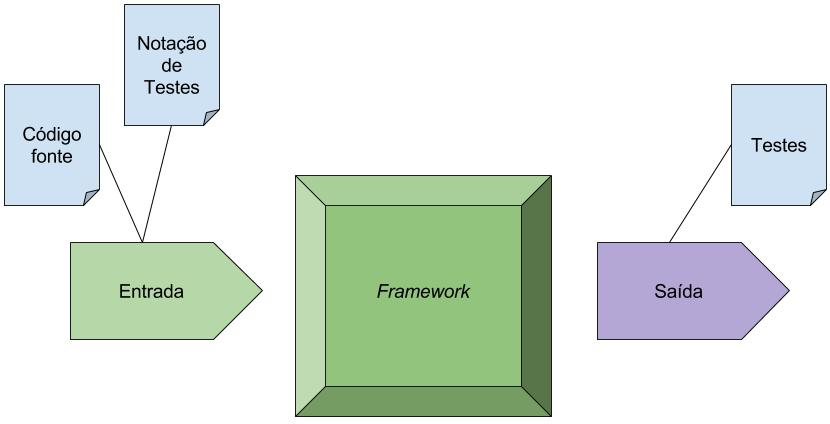
\includegraphics[width=0.7\textwidth]{figuras/entradasesaidas.jpg}
    \caption{Fluxo do funcionamento do \textit{Framework}}
    \label{fig:entradasesaidas}
 \end{figure}
 
 \par
\indent A Figura \ref{fig:entradasesaidas} enfatiza o fluxo do funcionamento do \textit{framework}. A entrada do \textit{framework} será o código fonte, bem como as especificações dos testes seguindo uma notação pré-determinada. Como saída, serão gerados os testes unitários conforme especifícados. O fluxo do funcionamento do \textit{framework} pode ser entendido, de forma simplificada, em quatro etapas: análise léxica, análise sintática, análise semântica e geração dos testes. 
 \begin{description}
 \item[Análise léxica:] onde será realizada a análise do código fonte de forma a reconhecer as palavras específicas, os \textit{tokens}. Essas palavras serão previamente definidas por meio do Flexc++ que fornece suporte para essa etapa \cite{flexcpp2015}.
 \item[Análise sintática:] ocorrerá uma avaliação do código fonte considerando as regras sintáticas definidas. Essas regras são formadas utilizando sequências de \textit{tokens}. Essa etapa será implementada com o auxílio do Bisonc++ cite{bisoncpp2015}.
 \item[Análise semântica:] será realizada uma interpretação do código apresentado verificando sua semântica, ou seja, será averiguado o significado dos \textit{tokens} identificados dentro do contexto.
  \item[Geração dos testes:] após as análises do código, será efetuado o \textit{parser} com o intuito de gerar os testes unitários específicados pelo desenvolvedor. Esses testes serão armazenados nos arquivos apropriados e serão a principal saída do \textit{framework}.
 \end{description}
 
 \begin{figure}[h]
    \centering
    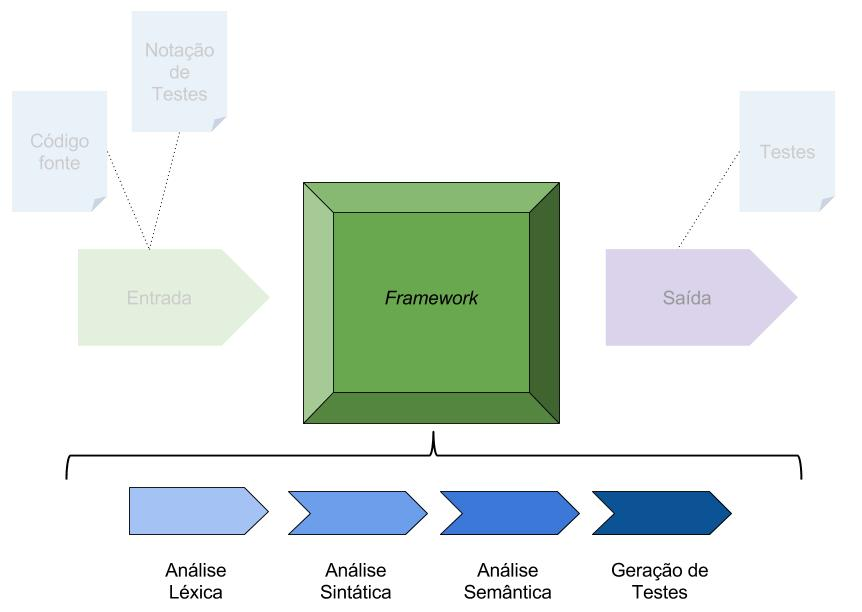
\includegraphics[width=0.9\textwidth]{figuras/Framework-interior.jpg}
    \caption{Fluxo do Funcionamento do \textit{Framework}}
    \label{fig:Framework-interior}
 \end{figure}
 
 \par
 \indent A Figura \ref{fig:Framework-interior} permite a visualização do fluxo básico do funcionamento do \textit{framework}. 

%% Como se dará a geração de teste
	%% Notação
	%% Arquitetura do framework
%% Qual será a saída
%% Sobre Grails
%%		Exemplo de teste e tals
%% 
%% Informações gerais sobre a condução do trabalho
\section{Prova de Conceito}

\section{Resultados Obtidos}
 
\section{Resumo do Capítulo}
%%  Resumo do capítulo

 